% LaTeX dokumentu guztiak zein dokumentu mota den adieraziz hasi behar dira
\documentclass[es]{ifirak}

% ERABILIKO DIREN PAKETEAK %

% listings paketea kodea formateatzeko erabiltzen da
\usepackage{listings}
% Paquete para los acentos
\usepackage[utf8]{inputenc}
\usepackage{colortbl}
\usepackage[table]{xcolor}
% Paketea konfiguratu behar dugu C lengoaiarekin erabiltzeko:
\definecolor{darkgreen}{rgb}{0,0.5,0}
\definecolor{lightgray}{rgb}{0.95,0.95,0.95}
\definecolor{gray}{rgb}{0.85,0.85,0.85}
\definecolor{white}{rgb}{1,1,1}
\definecolor{purple}{rgb}{0.51,0,0.25}
\definecolor{orange}{rgb}{0.255,0.178,0.102}

\lstdefinestyle{customc}{
	belowcaptionskip=1\baselineskip,
	breaklines=true,
	tabsize=4,
	language=C,
	showstringspaces=false,
	basicstyle=\footnotesize\ttfamily,
	keywordstyle=\bfseries\color{darkgreen},
	commentstyle=\itshape\color{purple},
	identifierstyle=\color{blue},
	stringstyle=\color{orange},
	backgroundcolor=\color{white},
}
\lstset{language=C++,escapechar=@,style=customc}

%\lstset{language=C++,
	%	basicstyle=\scriptsize\ttfamily,
	%	keywordstyle=\color{darkgreen}\bfseries,
	%	identifierstyle=\color{black},
	%	commentstyle=\color{gray}, 
	%	stringstyle=\ttfamily,
	%	showstringspaces=false,
	%	tabsize=2,
%	\textit{K}(\textit{m}, \textit{j}) = max \{ \textit{K}(\textit{m} - \textit{m_{j}}, \textit{j} - 1) + \textit{v_{j}} , \textit{K}(\textit{m}, \textit{j} - 1) \}
	%	backgroundcolor=\color{lightgray}}
%

\begin{document}
% Hainbat datu ...
\ikasturtea{2014 - 2015}
\irakasgaia{Diseño de algoritmos}
% Titulua
\title{Práctica de Programación 2}
% Zuen izena
\author{Mikel Dalmau}

\maketitle

% Abstract ingurunea hasierako laburpena idazteko erabili
\begin{abstract}
	\large{En la siguiente práctica se analizan el rendimiento de un algoritmo de fuerza bruta, backtrack, para el problema del viajante de comercio, se muestra como una poda inteligente puede mejorar sustancialmente el rendimiento .
}
\end{abstract}

% Testua egituratzeko section, subsection, subsubsection, subsubsection eta paragraph komandoak dituzue

\section{Enunciado del problema}

\large{
	\paragraph{}Es conocido que TSP es NP-completo, así que no es necesario un estudio analítico de la complejidad de tu algoritmo. Pero sí será interesante una explicación u justificación de las decisiones tomadas para intentar diseñar un algoritmo de backtrack inteligente.\\
	
	Se espera un estudio experimental que tome muestras del tiempo de ejecución de tu solución para una colección significativa de datos de prueba de tamaños distintos, y que presente esos datos en forma de tablas y gráficas.
	
}

\section{Estudio del problema y podas consideradas}

\subsection{Condiciones de satisfabilidad}
\large{
	\paragraph{}
	El problema del viajante de comercio consiste en encontrar el ciclo Hamiltoniano de menor coste.
	
	\begin{description}
		\item[Definición] Un ciclo Hamiltoniano en un grafo \textit{G}(\textit{V},\textit{E}) es un ciclo que contiene todos los vértices exactamente una vez.
		\item[Definición] Decimos que un grafo es Hamiltoniano si contiene un ciclo Hamiltoniano. Esto significa que al menos $|$\textit{V}$|$ $\geq$3 para que sea un grafo Hamiltoniano.\\
	\end{description}

	En muchos casos es imposible recorrer todos los nodos ya sea porque no haya caminos a estos o porque el grafo tiene más de un conjunto conexo. Si el número de nodos es muy grande puede ser conveniente realizar algunas comprobaciones previas a la ejecución del algoritmo, con la intención de determinar si no es satisfactible y ahorrarnos así realizar el cálculo de backtrack. 
	
	\begin{enumerate}
		\item Si existe algún nodo de grado 0 entonces el grafo no es conexo.
		\item Si existe algún nodo de grado 1 entonces es imposible realizar un ciclo Hamiltoniano.
		\item Si el grafo no es conexo no existe ciclo Hamiltoniano.
		\item Si el grafo es completo entonces también es Hamiltoniano.
	\end{enumerate}
	
	Para comprobar las primeras 2 condiciones basta con recorrer la matriz de adyacencia por filas sumando las aristas de cada nodo, en cuanto encontremos alguno de grado 0 o 1 se para y retorna el valor falso. El orden de esta comprobación es  $O(V^2)$.\\
	
	Aunque las primeras condiciones se cumplan puede ser que el grafo no sea conexo, basta con realizar una búsqueda en profundidad para determinarlo. El costo de esta operación es $O(V^2)$ también.\\
	
}

\large{
	\subsection{El algoritmo de Backtrack}
	\paragraph{}El algoritmo de Backtrack recorre el grafo probando todas las posibilidades de recorrer las ciudades hasta encontrar la óptima.\\ 
	
	Para abordar efectivamente el problema utilizando la técnica de backtracking definiremos el formato de los ensayos en primer lugar.\\
	
	Dado un grafo no dirigido \textit{G} con \textit{N} nodos y \textit{A} aristas representadas en una matriz de adyacencia \textit{adj}[\textit{N}][\textit{N}] donde los valores de la matriz indican el peso de cada arista.\\
	
	Sea \textit{R} una lista en la que están todos los nodos ya visitados colocados de forma ordenada, y sea \textit{S} otra lista en la que están el resto de nodos que quedan por visitar. Representaremos un ensayo como una lista con todos los nodos y un peso \textit{p}, así como un índice separador \textit{l} que dividirá la lista entre \textit{R} y \textit{S}. \\
	
	Para ampliar un ensayo miramos el último nodo de \textit{R} al que le corresponde la posición \textit{l} y buscamos un nodo entre los pertenecientes a \textit{S} tal que exista una arista entre los dos, esto es cuando \textit{adj}[\textit{l}][\textit{i}] con $l<i<N$, es un entero válido.\\
	
	Identificamos un ensayo como casi una solución cuando \textit{l} = N-1 esto significa que $R = \{V\}$ y $S=\{\phi\}$ solo queda una arista por completar, la que une el último nodo con el primero completando así el ciclo del viajante de comercio. Sólo si esta arista existe el ensayo es solución.\\ 
	
	No es válido un ensayo cuando el último nodo de \textit{R} no tenga aristas a ningún nodo de \textit{S}, entonces el algoritmo de backtrack ignora este caso no realizando ninguna llamada recursiva, en definitiva, no puede ampliarse el ensayo.\\
	\vspace*{1.5cm}
	\pagebreak
	
	\begin{figure}[htbp]
		\begin{tabular}{lccccc}                                                            
			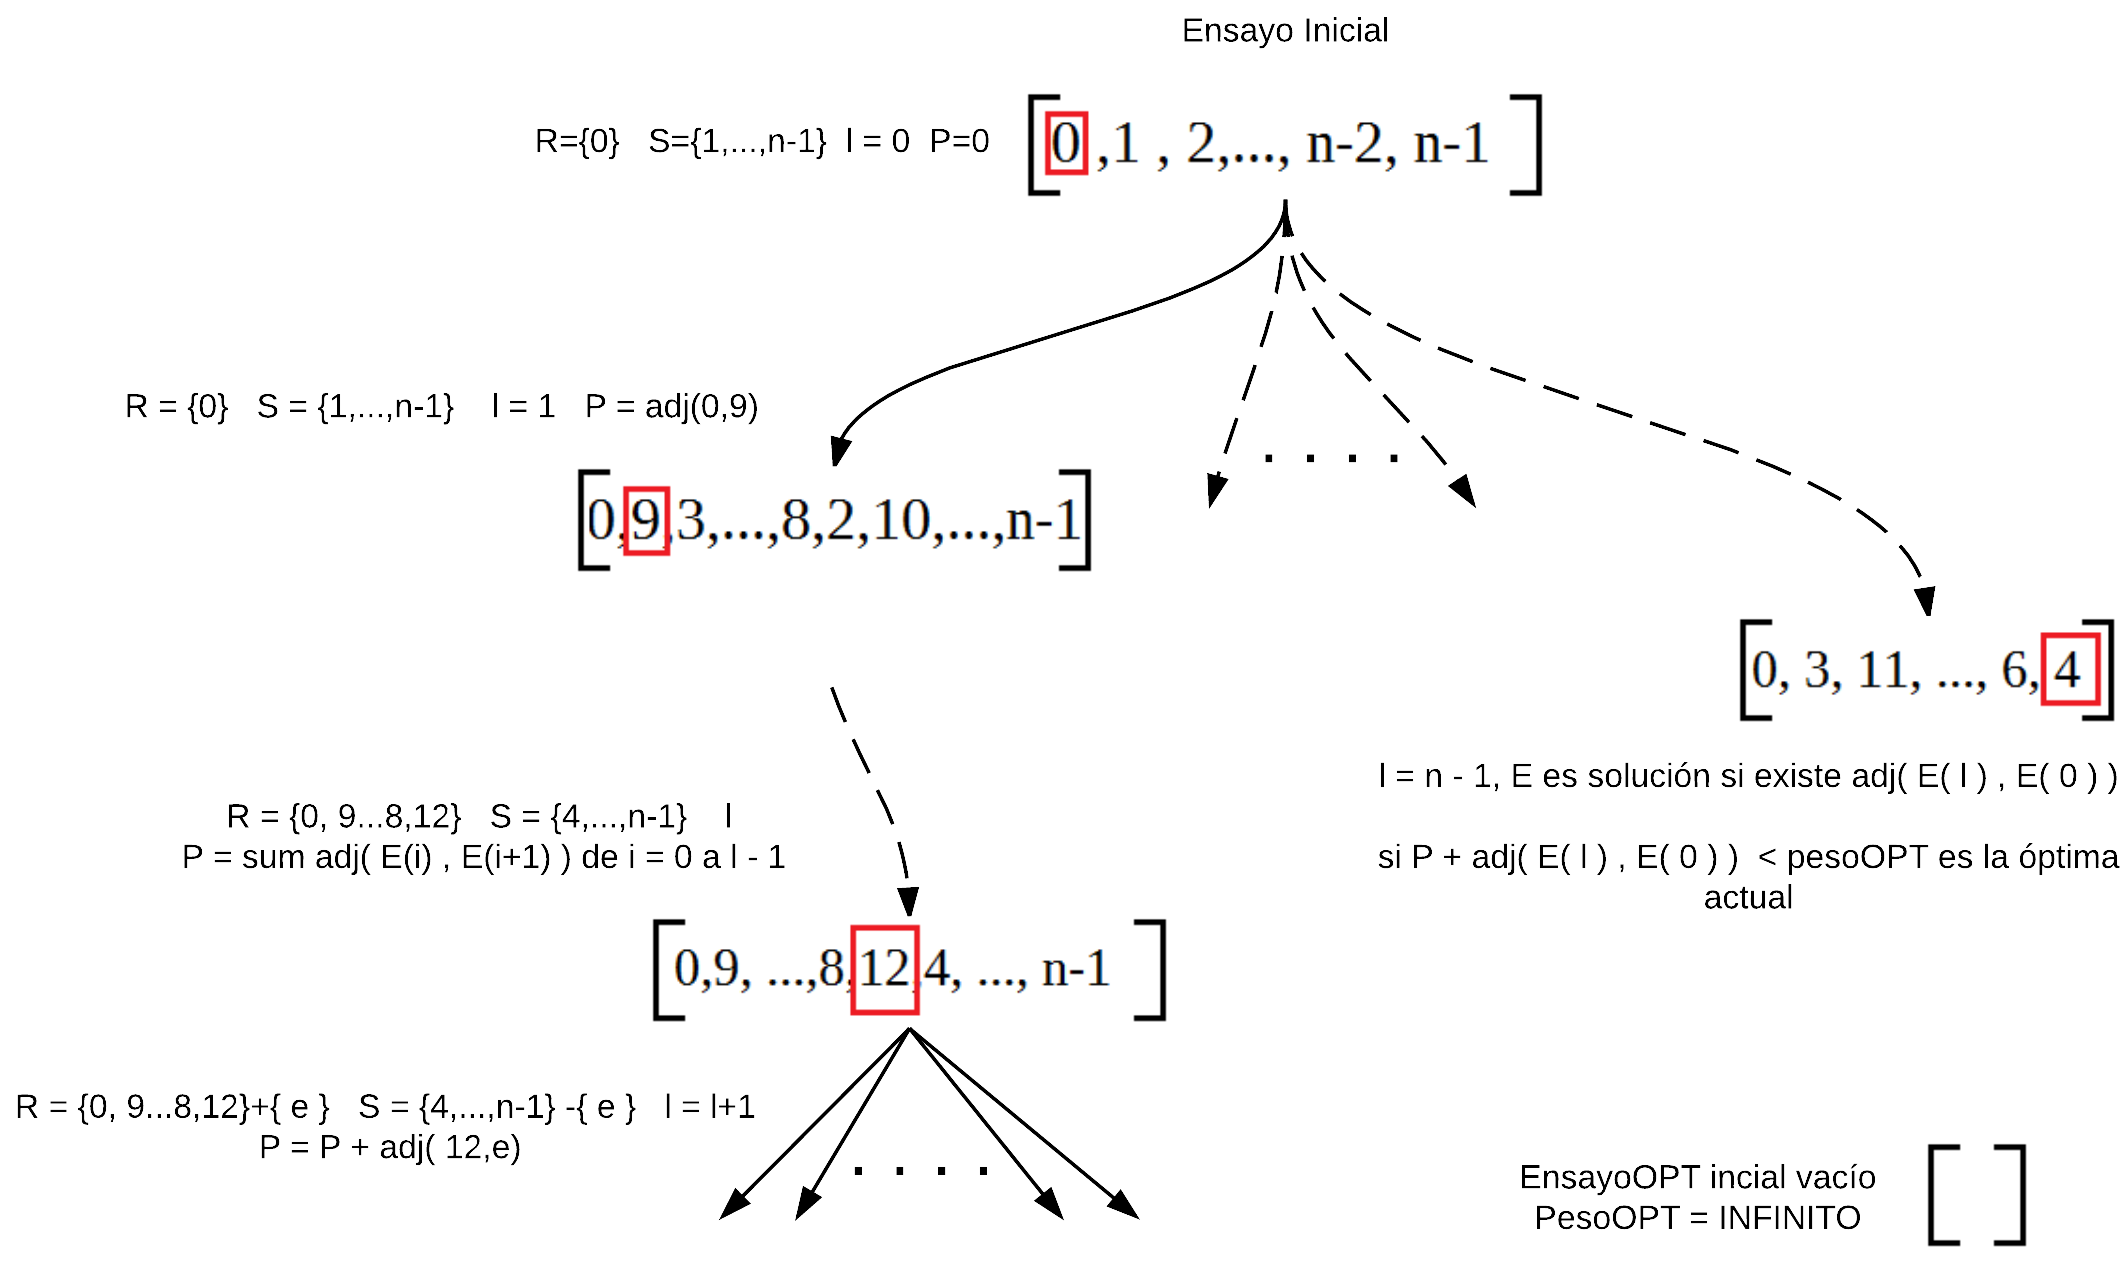
\includegraphics[width=1\textwidth]{Arbol_ensayos_Backtrack.png}& \hspace*{ 4cm}&   &   &   &                                       
		\end{tabular}
		\caption{Representación del árbol de ensayos.}\label{figure}
	\end{figure}
	
	
	\pagebreak
	\subsection{Backtrack ingenuo}
	\paragraph{}
	Esta es la implementación más básica del algoritmo Backtrack para el problema del Viajante de Comercio, se prueban todos los caminos válidos del grafo y tiene orden $O(n!)$.\\
	
	\textbf{Algoritmo} TSP\_Backtrack (E, l , dist, adj(n)(n) )\\
\hspace*{0.8cm}	 n = longitud(E) \\	
\hspace*{0.8cm}	\textbf{si} l = n-1 \textbf{entonces}\\ 
\hspace*{0.4cm}\hspace*{2cm}	\textbf{si} existe arista E(n) $\leftrightarrow$ E(0) \textbf{entonces}\\
\hspace*{0.4cm}\hspace*{2.6cm}	 minCost $\leftarrow$ dist + adj(E(n),E(0)) \\
\hspace*{0.8cm}	\textbf{si no} minCost $\leftarrow$ $ \infty$\\
\hspace*{0.4cm}\hspace*{2cm}	\textbf{desde} i $\leftarrow$ l+1 \textbf{hasta} n\\
\hspace*{0.4cm}\hspace*{2cm}	\textbf{si} existe arista A(l) $\leftrightarrow$ E(i) \textbf{entonces}\\ 
\hspace*{0.4cm}\hspace*{2.6cm}	nuevadist $\leftarrow$ dist + adj(E(l),E(i))\\
\hspace*{0.4cm}\hspace*{2.6cm}	intercambiar E(l+1) y E(i)\\
\hspace*{0.4cm}\hspace*{2.6cm}	minCost  $\leftarrow$ min\{ minCost, TSP\_Backtrack (E, l+1 , nuevadist, adj) \}\\
\hspace*{0.4cm}\hspace*{2.6cm}	intercambiar E(l+1) y E(i)\\
\hspace*{0.8cm}	\textbf{return} minCos\\
	
	\subsection{Backtrack acotado}
	
	El siguiente algoritmo es equivalente al anterior pero añade una restricción que impide ampliar ensayos que superen en peso al ensayo óptimo, si es que este existe.
	
	\textbf{Algoritmo} TSP\_Backtrack(E, l, dist, adj(n)(n) )\\
	\hspace*{0.8cm}	 n = longitud(E) \\	
	\hspace*{0.8cm}	\textbf{si} l = n-1 \textbf{entonces}\\ 
	\hspace*{0.4cm}\hspace*{2cm}	\textbf{si} existe arista E(n) $\leftrightarrow$ E(0) \textbf{entonces}\\
	\hspace*{0.4cm}\hspace*{2.6cm}	 minCost $\leftarrow$ dist + adj(E(n),E(0)) \\
	\hspace*{0.8cm}	\textbf{si no} minCost $\leftarrow$ $ \infty$\\
	\hspace*{0.4cm}\hspace*{2cm}	\textbf{desde} i $\leftarrow$ l+1 \textbf{hasta} n\\ 
	\hspace*{0.4cm}\hspace*{2cm}	\textbf{si} existe arista E(l) $\leftrightarrow$ E(i) \textbf{entonces}\\
	\hspace*{3cm}	nuevadist $\leftarrow$ dist + adj(E(l),E(i))\\
	\hspace*{3cm} \textcolor{purple}{\textbf{si} nuevadist $<$ minCost \textbf{entonces}}\\
	\hspace*{3.6cm}	intercambiar E(l+1) y E(i)\\
	\hspace*{3.6cm}	minCost  $\leftarrow$ min\{minCost,  TSP\_Backtrack (E, l+1 , nuevadist, adj)\}\\
	\hspace*{3.6cm}	intercambiar E(l+1) y E(i)\\
	\hspace*{0.8cm}	\textbf{return} minCos\\
	
	\pagebreak
	\subsection{El mejor el primeroS}
	\paragraph{}
	El algoritmo Best First o el Mejor el Primero, prueba también todos los ensayos posibles, pero en vez de ampliar siempre el mismo ensayo, haciendo un recorrido en profundidad, este algoritmo amplía el ensayo de menor peso entre los que disponemos. Lo que hace es guardar en una estructura de montículo los ensayos y así retiramos siempre el de menor peso. Cabe resaltar que cuando un ensayo es solución, se guarda en el montículo también, solo cuando cuando retiramos la cima del montículo y es solución entonces es la óptima ya que todos los ensayos restantes tienen mayor peso.\\
	
		\textbf{Algoritmo} TSP\_MejorPrimero(E, adj(n)(n) )\\
		\hspace*{0.8cm}	 \textbf{crear} montículo\\ 
		\hspace*{0.8cm}	 montículo \textbf{insertar} E\\ 
		\\ 
		\hspace*{0.8cm}	 \textbf{mientras} !fin \\	
		\hspace*{0.6cm}\hspace*{0.8cm}  montículo \textbf{eliminarCima}\\ 
\hspace*{0.6cm}	\hspace*{0.8cm}	 l $\leftarrow$ E.l \\	
\\ 
	\hspace*{0.6cm}	\hspace*{0.8cm}	\textbf{si} l = n \textbf{entonces}\\ 
\hspace*{0.6cm}		\hspace*{0.4cm}\hspace*{2cm} \textbf{return} E\\
\hspace*{0.6cm}		\hspace*{0.8cm}	\textbf{si} l = n - 1 \textbf{entonces}\\ 
\hspace*{0.6cm}		\hspace*{2.4cm}	\textbf{si} existe arista E(n) $\leftrightarrow$ E(0) \textbf{entonces}\\
\hspace*{0.6cm}		\hspace*{3cm}	 E.peso $\leftarrow$ E.peso + adj(E(n),E(0)) \\ 
\hspace*{0.6cm}		\hspace*{3cm}	 E.l  $\leftarrow$ n \\	
\hspace*{0.6cm}		\hspace*{3cm}	\textbf{si}  E.peso  $<$ minCost \textbf{entonces}\\
\hspace*{0.6cm}		\hspace*{3.6cm} monticulo \textbf{insertar} E\\
\hspace*{0.6cm}		\hspace*{3.6cm} monticulo \textbf{eliminar mayores}(E.peso) \\
\hspace*{0.6cm}		\hspace*{0.8cm}	\textbf{si no} \\
\hspace*{0.6cm}		\hspace*{2.4cm}	\textbf{desde} i $\leftarrow$ l+1 \textbf{hasta} n\\ 
\hspace*{0.6cm}	\hspace*{0.6cm}	\hspace*{2.4cm}	\textbf{si} existe arista E(l) $\leftrightarrow$ E(i) \textbf{entonces}\\
\hspace*{0.6cm}	\hspace*{0.6cm}	\hspace*{3cm}	nuevadist $\leftarrow$ E.peso + adj(E(l),E(i))\\
\hspace*{0.6cm}	\hspace*{0.6cm}	\hspace*{3cm} \textbf{si} nuevadist $<$ minCost \textbf{entonces}\\
\hspace*{0.6cm}	\hspace*{0.6cm}	\hspace*{3.6cm}	 E.peso $\leftarrow$ nuevadist \\	
\hspace*{0.6cm}	\hspace*{0.6cm}	\hspace*{3.6cm}	 E.l  $\leftarrow$ l + 1 \\	
\hspace*{0.6cm}	\hspace*{0.6cm}	\hspace*{3.6cm}	intercambiar E(l+1) y E(i)\\
\hspace*{0.6cm}	\hspace*{0.6cm}	\hspace*{3.6cm}	monticulo \textbf{insertar} E\\
\hspace*{0.6cm}	\hspace*{0.6cm}	\hspace*{3.6cm}	intercambiar E(l+1) y E(i)\\
\hspace*{0.6cm}	\hspace*{0.6cm}	\hspace*{3.6cm}	 E.l  $\leftarrow$ l - 1 \\	
\hspace*{0.6cm}	\hspace*{0.6cm}	\hspace*{3.6cm}	 E.peso $\leftarrow$ antiguadist\\	
\\
\hspace*{1.4cm}	\textbf{si} monticulo es vacío \textbf{entonces}\\ 		
		\hspace*{2cm} fin  $\leftarrow$ verdadero \\
\hspace*{1.4cm}	\textbf{si no}\\
 \hspace*{2cm} E $\leftarrow$ montículo \textbf{extraerCima}\\ 
}

\pagebreak

\section{Estudio experimental}

En la siguiente sección se muestran los tiempos de cada algoritmo para distintos tamaños de fichero. Los ficheros utilizados son grafos completos de N nodos A aristas, y todos ellos son satisfactibles por ser completos. Es el peor escenario posible para N nodos, en el caso de backtrack ingenuo por ejemplo el orden sería $\Theta(n!)$ ya que probaría exactamente todas las posibilidades. En los otros casos el orden es $O(n!)$.\\

Cabe destacar que los tiempos para el algoritmo Best First son mayores que para el Backtrack acotado, es posible que esto sea debido a la gestión del montículo que añade esas operaciones extra, sería interesante, aunque no he tenido tiempo de realizar las pruebas, ver si para tamaños de entrada mayores el algoritmo Best First supera al acotado.

\paragraph{}
\begin{center}
	\begin{table}[htbp]
		\centering
		\begin{tabular}{|c|c|c|c|c|}
		\hline
		\cellcolor{gray}	N & \cellcolor{gray}A & \cellcolor{gray}BT Ingenuo &\cellcolor{gray} BT Acotado &\cellcolor{gray} BT BestFirst \\
		\hline
		7 & 36 & 0.016     & 0		& 0  	\\
		8 & 45 & 0.14      & 0		& 0		\\
		9 & 55 & 1.358     & 0.015	& 0.031	\\
		10 & 66 & 28.392   & 0.032	& 0.062	\\
		11 & 78 & 324.606  & 0.269	& 1.809	\\
		12 & 91 &  4519.78 & 0.109	& 0.998	\\
		13 & 105 &  ...    & 0.5	& 3.167	\\
		14 & 120 &  ...    & 2.87	& 26.739	\\
		15 & 136 & 	...	   & 9.766	& 58.952	\\
		16 & 153 & 	...	   & 81.073	& 974.912	\\
		\hline
		\end{tabular}
		\caption{Tabla de tiempos de ejecución.}\label{table}
	\end{table}
\end{center}


\begin{figure}[htbp]
	\centering
	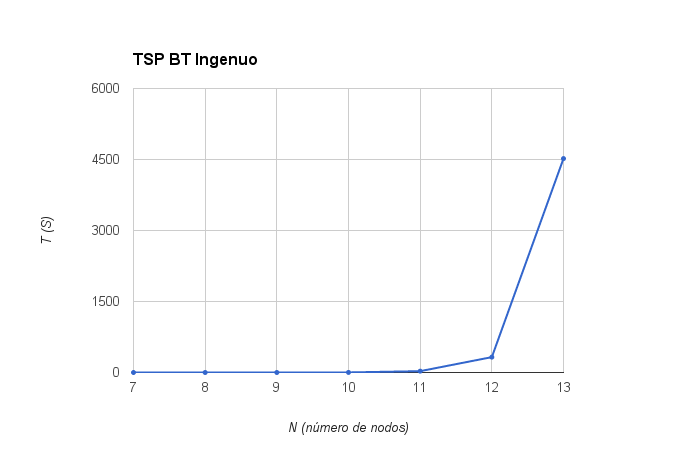
\includegraphics[width=0.9\textwidth]{BTING.png}
	\caption{Representación gráfica de la columna BT Ingenuo de la tabla 1. }\label{figure}
\end{figure}

\begin{figure}[htbp]
	\centering
	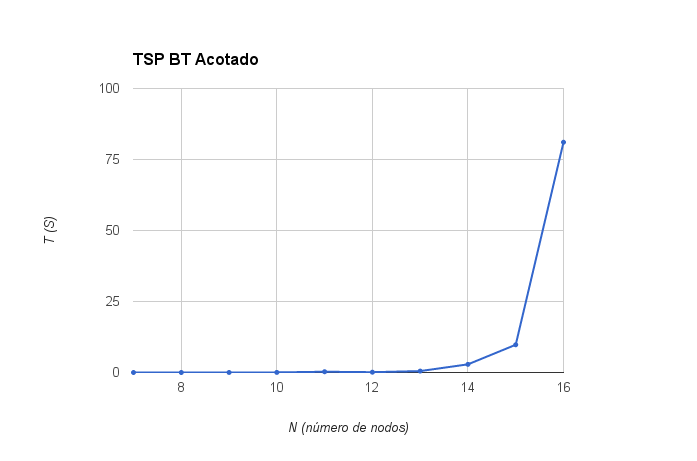
\includegraphics[width=0.9\textwidth]{BTAC.png}
	\caption{Representación gráfica de la columna BT Acotado de la tabla 1.}\label{figure}
\end{figure}

\begin{figure}[htbp]
	\centering
	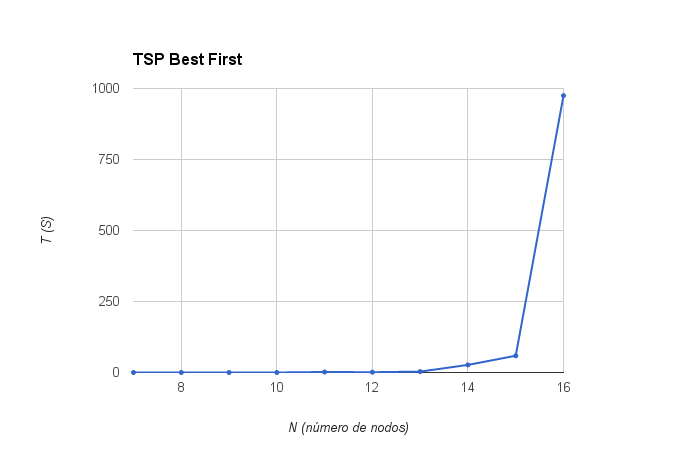
\includegraphics[width=0.9\textwidth]{BTBF.png}
	\caption{Representación gráfica de la columna BT BestFirst de la tabla 1.}\label{figure}
\end{figure}

\begin{figure}[htbp]
	\centering
	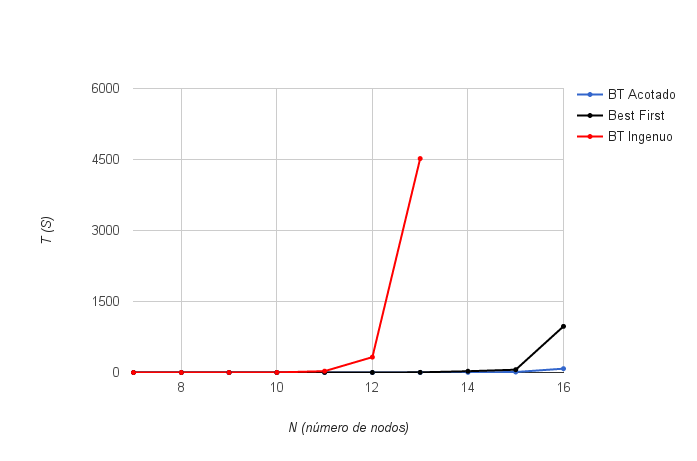
\includegraphics[width=0.9\textwidth]{BTTODOS.png}
	\caption{Representación gráfica de la tabla 1.}\label{figure}
\end{figure}

\paragraph{}

\pagebreak

\begin{thebibliography}{arauak}
	
	\bibitem[cppRef]{key-1} http://es.cppreference.com .
	
	\bibitem[win.tue]{key-2} http://www.win.tue.nl/~kbuchin/teaching/2IL15/backtracking.pdf
	
	\bibitem[Das]{key-3} Algorithms, S. Dasgupta, C. H. Papadimitriou, and U. V. Vazirani.
	
	\bibitem[prince]{key-4}http://www.cs.princeton.edu/courses/archive/spr08/cos226/assignments/backtrack.html
	
	\bibitem[man]{key-5} http://www.maths.manchester.ac.uk/~mrm/Teaching/DiscreteMaths/LectureNotes/HamiltonBondyAndChvatal.pdf
	
\end{thebibliography}

\section{Anexo}
	\subsection{Comentarios}
		\paragraph{}
		He dedicado muchas horas a trabajar en esta práctica pero me he centrado demasiado quizá en la implementación de los algoritmos y no he dedicado el tiempo suficiente a realizar las pruebas. Por esto no he podido obtener datos de ejecuciones para ficheros más grandes, alrededor de 19 o 20 nodos habría sido ideal. 
	\subsection{Teorema de Bondy-Chvátal}
	\large{
		\paragraph{}
		Este Teorema demostrado por J. Adrain Bondy y Vasek Chvátal viene a decir en esencia que si un grafo tiene muchas aristas, entonces tiene que ser Hamiltoniano. Puede leerse la demostración de este teorema en \cite{key-5}. 
		\begin{description}
			\item[Teorema] (Bondy-Chvátal,1976) \textit{Un grafo \textit{G} es Hamiltoniano si y solo si su cerradura $[G]$ es Hamiltoniano.}
		\end{description}
		
		La cerradura de un grafo \textit{G} de n vértices, $[G]$, se construye añadiendo aristas a los pares de vértices no adyacentes \textit{u} y \textit{v} para los que:
		$$ grado(u) + grado(v) \geq n$$
		\paragraph{}
		Se continua agregando aristas recursivamente hasta que todos los vértices no adyacentes cumplan:
		$$ grado(u) + grado(v) < n$$
		\paragraph{}	
		Los grafos G y $[G]$ tienen los mismos vértices pero el conjunto de aristas de $[G]$ puede contener aristas añadidas.
		
		Los siguientes teoremas se obtienen ambos como corolario del teorema de Bondy-Chvátal. 
		\begin{description}
			\item[Teorema] (Dirac, 1952) \textit{Sea \textit{G} un grafo con n $\geq$3. Si cada vértice de G tiene grado(v)$\geq$n/2 entonces \textit{G} es Hamiltoniano.}
			\item[Teorema] (Ore, 1960) Sea \textit{G} un grafo con n $\geq$3. Si,
			$$ grado(u) + grado(v) \geq n$$ para cada par de vértices no adyacentes u y v, entonces \textit{G} es Hamiltoniano.
		\end{description}
		\paragraph{}
		Aunque en la práctica no me sirvió de nada ya que solo vale para demostrar que un grafo es Hamiltoniano y al fin y al cabo yo debía hallar el ciclo óptimo, ha sido una buena experiencia poder programar la cerradura de un grafo y las condiciones expuestas, es posible que en algún contexto nos interesara saber solamente si un grafo tiene solución.
	}
	
\subsection{Código}
\paragraph{}
Las siguientes páginas contienen todo el código utilizado, en lenguaje c++.
\begin{lstlisting}

/* 
* File:   main.cpp
* Author: mikel
*
* Created on 7 de mayo de 2015, 17:02
*/
#include <vector>
#include <cstdlib>
#include <iostream>
#include <fstream>
#include <cmath>
#include <time.h>
#include <string.h>
#include <limits>
#define INFINITO -1
#define DEFAULT -1
#define INGENUO 0
#define ACOTADO 1
#define BESTFIRST 2
#define PRE_CONEXO 1
#define PRE_GRADO 0
#define PRE_GRADO_CONEXO 2
#define PRE_BOND_CHVA 3

#include "MinHeap.h"

using namespace std;

clock_t tic,toc;

typedef struct {
	int** pesos;
	vector<int> grado;
	int N;
	int A;
}grafo;

//Definicion movida a MinHeap.h
//typedef struct {
//  int peso;
//  vector<int> nodos;
//  int l;
//}ensayo;

void crearGrafoCompleto(int n, string fname);
bool OreCond(grafo *G);
bool DiracCond(grafo *G);
bool esCompleto(grafo *G);
grafo cerradura(grafo G);
bool contarGradoVertices(grafo *G);
void visita(grafo *G,vector<bool> *pV, int nodo);
bool conexo(grafo *G);
void swap(ensayo *pE, int i, int j);
int leerFichero(string pFname, grafo *pG);
void imprimirMatriz(grafo *G);
ensayo TSP_Backtrack_Acotado(grafo *G,ensayo E,ensayo Eopt,int l);
ensayo TSP_Backtrack_Ingenuo(grafo *G,ensayo E,ensayo Eopt,int l);
ensayo TSP_Backtrack_PrimeroMejor(grafo *G,ensayo Einicial);
void TSP(string pFname, int TIPOALG, int PREPROC);
int main(int argc, char** argv);

int main(int argc, char** argv) {  

//Espacio Para hacer las pruebas pertinentes

return 0;
}
void TSP(string pFname, int TIPOALG, int PREPROC){
	grafo G; 
	ensayo E,Eopt; 
	int N =  leerFichero(pFname,&G);
	bool satisf = true;   
	
	switch (PREPROC){
	
	case PRE_GRADO:
		satisf = contarGradoVertices(&G);
		break;
	
	case PRE_CONEXO:
		satisf = conexo(&G);
		break;
	
	case PRE_GRADO_CONEXO:
		satisf = contarGradoVertices(&G);
		satisf = conexo(&G);
		break;
	
	case  PRE_BOND_CHVA:
		if (!contarGradoVertices(&G)){satisf = false;}
		else{ 
			if (!conexo(&G)){satisf = false;} 
			else{
				grafo cG =cerradura(G);
				if(esCompleto(G)){satisf = true;}
				if(OreCond(G)){satisf = true;}
				if(DiracCond(G)){satisf = true;}
			}
		} 
		break;
	
	default:
		break;
	}
	
	if(satisf){
		/*
		* Construimos el ensayo inicial
		*/
		E.peso = 0; E.l=0;
		E.nodos = vector<int>(G.N);
		for(int i = 0; i < G.N ; i++)
			E.nodos[i] = i;
			
		Eopt.peso = INFINITO;
		Eopt.nodos = vector<int>(G.N);
	
	switch (TIPOALG){
	
		case INGENUO:
			Eopt = TSP_Backtrack_Ingenuo(&G,E,Eopt,0);
			break;
		
		case ACOTADO:
			Eopt = TSP_Backtrack_Acotado(&G,E,Eopt,0);
			break;
		
		case BESTFIRST:
			Eopt = TSP_Backtrack_PrimeroMejor(&G,E);
			break;
		
		default:
			cout << "Algoritmo seleccionado incorrecto" << endl ; return;
			break;
	}
	
	if(Eopt.peso != INFINITO){
		for(int j= 0; j< Eopt.nodos.size(); j++)
			cout << Eopt.nodos[j] << " ";
		cout << endl << " Peso del recorrido: " << Eopt.peso  << endl; return;  
	}
		}   
	cout << "Insatisfactible" << endl ; return;
};

ensayo TSP_Backtrack_Ingenuo(grafo *G,ensayo E,ensayo Eopt,int l){
	int n = G->N;
	
	if( n-1 == l){
	if(G->pesos[ E.nodos[n-1] ][ E.nodos[0] ] != INFINITO){
		Eopt.peso = E.peso + G->pesos[ E.nodos[n-1] ][ E.nodos[0] ];
		Eopt.nodos.operator =(E.nodos);     
	}
	}else{
		Eopt.peso=INFINITO;
		int antiguoPeso = E.peso;
		
		for(int i = l+1; i < n; i++)
			if( G->pesos[ E.nodos[l] ][ E.nodos[i] ] != INFINITO){          
				int nuevoPeso = E.peso + G->pesos[ E.nodos[l] ][ E.nodos[i] ];
				E.peso = nuevoPeso;
				swap(&E,l+1,i);    
				ensayo Eaux = TSP_Backtrack_Ingenuo(G,E,Eopt,l+1);
				if(Eopt.peso == INFINITO){
					if(Eaux.peso != INFINITO){  Eopt = Eaux;}   
				}else{
					if(Eaux.peso != INFINITO and Eaux.peso < Eopt.peso){ Eopt = Eaux; }   
				}
				swap(&E,i,l+1);
				E.peso = antiguoPeso;
			}
	}
	return Eopt;
};

ensayo TSP_Backtrack_Acotado(grafo *G,ensayo E,ensayo Eopt,int l){
	int n = G->N;
	
	if( n-1 == l){ 
		if(G->pesos[ E.nodos[n-1] ][ E.nodos[0] ] != INFINITO){ 
			if(Eopt.peso == INFINITO){
				Eopt.peso = E.peso + G->pesos[ E.nodos[n-1]][E.nodos[0] ];
				Eopt.nodos.operator =(E.nodos);  
			}else{
				if(E.peso + G->pesos[ E.nodos[n-1]][ E.nodos[0] ] < Eopt.peso){
					Eopt.peso = E.peso + G->pesos[ E.nodos[n-1]][ E.nodos[0] ];
					Eopt.nodos.operator =(E.nodos);  
				}   
			}
		}
	}else{
	int antiguoPeso = E.peso;
	
	for(int i = l+1; i < n; i++)
		if(G->pesos[ E.nodos[l] ][ E.nodos[i] ] != INFINITO){
			int nuevoPeso = E.peso + G->pesos[ E.nodos[l] ][ E.nodos[i] ];
			if(Eopt.peso==INFINITO or nuevoPeso < Eopt.peso){
				E.peso = nuevoPeso;
				swap(&E,l+1,i);    
				ensayo Eaux = TSP_Backtrack_Acotado(G,E,Eopt,l+1);
				if(Eopt.peso == INFINITO){
					if(Eaux.peso != INFINITO){  Eopt = Eaux;}   
				}else{
					if(Eaux.peso != INFINITO and Eaux.peso < Eopt.peso){  Eopt = Eaux;  }   
				}
				swap(&E,i,l+1);
				E.peso = antiguoPeso;
				}
			}
		}
	return Eopt;
};

ensayo TSP_Backtrack_PrimeroMejor(grafo *G,ensayo Einicial){
	ensayo E; int n = G->N; bool fin = false;
	int pesoOPT  = INFINITO;
	
	ensayo e[] = {Einicial};
	MinHeap monticulo = MinHeap(e,1);
	E  = monticulo.GetMin();
	
	while(!fin){ 
		monticulo.DeleteMin();
		int l = E.l;
		
		if( l ==  n ) {
			return E;
		
		}else if( l == n-1 ) {
			if(G->pesos[ E.nodos[n-1] ][ E.nodos[0] ] != INFINITO){ 
				E.peso = E.peso + G->pesos[ E.nodos[n-1] ][ E.nodos[0] ];
				E.l = n;
				if(pesoOPT == INFINITO or E.peso < pesoOPT){
					pesoOPT = E.peso;
					monticulo.Insert(E);
					monticulo.DeleteFrom(pesoOPT);
				}
			}
		}else{
			int antiguoPeso = E.peso; 
			for(int i = l+1; i < n; i++)
				if( G->pesos[ E.nodos[l] ][ E.nodos[i] ] != INFINITO){          
					int nuevoPeso = antiguoPeso + G->pesos[ E.nodos[l] ][ E.nodos[i] ];
					if(pesoOPT==INFINITO or nuevoPeso < pesoOPT){
						E.peso = nuevoPeso;
						swap(&E,l+1,i);    
						E.l = l + 1;
						monticulo.Insert(E);
						E.l= l - 1; 
						swap(&E,l+1,i); 
					}   
				}
		}
		if(monticulo.isEmpty()){ fin = true; }
		else{E = monticulo.GetMin();}
	}
	return E;
};

grafo cerradura(grafo G){
	grafo cG; 
	
	cG.A = G.A; cG.N = G.N;
	cG.grado=G.grado; 
	int** pesos;
	pesos = new int* [cG.N]; 
	for (int j = 0; j < cG.N; j++){   
		pesos[j] = new int [ cG.N]; 
		for(int h=0; h<  cG.N ; h++)
			pesos[j][h] = G.pesos[j][h];
	}
	cG.pesos=pesos;
	
	int i,j;
	bool finished = false;
	bool seAgregaArista = false;
	while(!finished){
		i = 0;
		seAgregaArista = false;
		while( i < cG.N and !seAgregaArista){
			j = 0;
			while( j < cG.N and !seAgregaArista){
				if(cG.pesos[i][j] == INFINITO and i!=j)
					if(cG.grado[i] + cG.grado[j] >= cG.N){
						cG.pesos[i][j] = 1;
						cG.pesos[j][i] = 1;
						cG.grado[i]++;
						cG.grado[j]++;
						seAgregaArista = true;
					}
				j++;
			}
			i++;
		}
		if(!seAgregaArista)
			finished = true;
	}
	return cG;
};

void swap(ensayo *pE, int i, int j){
	if(i < 0 or i > pE->nodos.size()){  return; }
	if(j < 0 or j > pE->nodos.size()){  return; }
	
	int swap = pE->nodos[j];
	pE->nodos[j] = pE->nodos[i];
	pE->nodos[i] = swap;
};

bool conexo(grafo *G){
	vector<bool> visitados(G->N);
	visita(G,&visitados,0);
	for(int i=0; i<G->N; i++)
		if(visitados[i]==false){
			return false;
		}
	return true;
};

void visita(grafo *G,vector<bool> *pV, int nodo){
	pV->at(nodo)=true;
	for(int i= 0; i<G->N; i++){
		if(G->pesos[nodo][i] != INFINITO and pV->at(i)==false){
			visita(G,pV,i);
		}
	}
};

bool contarGradoVertices(grafo *G){
	G->grado=vector<int>(G->N);
	for(int i=0; i<G->N; i++){
		int grado = 0;
		for(int j=0;j<G->N;j++)
			if(G->pesos[i][j] != INFINITO)
				grado++;
		G->grado[i]=grado;
		if(grado < 2){
			return false;
		}
	}
	return true;
};

bool esCompleto(grafo *G){
	for(int i=0; i<G->grado.size();i++)
		if( G->grado[i] != G->N)
		return false;
	return true;
};

bool DiracCond(grafo *G){
	for(int i=0; i<G->grado.size();i++)
	if( G->grado[i] <= G->N/2 )
		return false;
	return true;
};

bool OreCond(grafo *G){
	for(int i=0; i<G->N; i++)
		for(int j=0; j<G->N; j++)
			if(G->pesos[i][j] == INFINITO and i!=j)
				if( G->grado[i] +G->grado[j] < G->N)
					return false;
	return true;
};

int leerFichero(string pFname, grafo *pG){
	int i=0,origen,destino,peso;
	grafo G;
	const int anInt = sizeof(anInt);
	char cadena[500];
	ifstream fe(pFname.c_str());
	
	for(int h = 0; h < 5; h++){
		fe.getline(cadena, 500);
	}
	fe >> G.N; fe >>  G.A;
	int** pesos;
	pesos = new int* [ G.N]; 
	for (int j = 0; j < G.N; j++){   
		pesos[j] = new int [ G.N]; 
		for(int h=0; h<  G.N ; h++)
			pesos[j][h] = INFINITO;
	}
	
	for(i = 0; i < G.A ; i++){
		fe >> origen;
		fe >> destino;
		fe >> peso;
		pesos[origen][destino] = peso;
		pesos[destino][origen] = peso;
	}
	fe.close();
	G.pesos = pesos;
	*pG = G;
	return G.N;
};

void imprimirMatriz(grafo *G){
	for(int i = 0; i < G->N; i++){
		for(int j = 0; j < G->N; j++)
			cout << G->pesos[i][j] <<  "\t";  
		cout << endl;
	}
};
void crearGrafoCompleto(int n, string fname){
	ofstream fe(fname.c_str());
	int coste; int A= 0;
	for(int k = n ; k > 0; k--){A = A + k;}
	
	fe << "c" << endl;  fe << "c" << endl;  fe << "c" << endl; fe << "c" << endl; fe << "c" << endl;
	
	fe << n << " " << A << endl;
	for(int i = 0; i < n; i++)
		for(int j= i; j < n; j++){
			coste = 1 + (rand() % 30);
			if(j == i){
				fe << i << " " << j << " -1" << endl;
			}else{
				fe << i << " " << j << " " <<coste << endl;
			}
		}           
	fe.close();
}
\end{lstlisting}

\end{document}
